\documentclass[10pt,a4paper]{article}
\usepackage[utf8]{inputenc}
\usepackage{amsmath}
\usepackage{amsfonts}
\usepackage{amssymb}

\author{Carl Svensson carlsven@kth.se \& Erik Larsson erikl3@kth.se}
\title{El Gamal Mixnets and Implementation of a Verifier \\ SA104x Degree Project in Engineering Physics \\
KTH Royal Institute of Technology \\
School of Computer Science and Communication
Supervisor: Douglas Wikström}
\begin{document}

\maketitle
\tableofcontents

\setlength{\parindent}{0pt}
\setlength{\parskip}{10pt plus 1pt minus 1pt}

\pagebreak
\begin{frame}{Häftigt med riksdagsval}

\begin{itemize}
\item Rösta snabbt/säkert/hemligt
\item Verifierbart
\item Robust
\item Kanske ingen valvaka
\end{itemize}

\end{frame}
\subsection{El Gamal Cryptography}

The El Gamal cryptosystem is based on group theory, to which a short
introduction is provided in Appendix A. In full generality, a public
key cryptosystem, or an assymetric cryptosystem, provides two parties
the means to communicate privately without the need of sharing a
common secret beforehand as is the case in symmetric cryptography
(källa). The cryptosystem consists of a public key, a secret key and
two functions - one encryption function which uses the public key and
one decryption function which uses the secret key (källa).

In the El Gamal cryptosystem the communicating parties agrees on a
cyclic group and a generator element. The secret key is an integer,
while the public key is a group element - the exponentation of the
generator by the secret key integer (källa). Encryption of a message
(note that the messages need to be encoded into elements of the group)
is done by multiplying the message with a group element that has a
special relation to the public key. Now, only the possessor of the
secret key can decrypt, since without the key it is unfeasible to
invert this multiplication. This is a slight simplification, but it
should capture the main idea of the cryptosystem.

Every asymmetric cryptosystem depends on the assumption that there
exist computationally difficult problems. This is the case also for
the El Gamal cryptosystem for which the security depends on the
difficulty of deducing information about the discrete logarithm in a
cyclic group (källa).

As we shall see, the El Gamal cryptosystem possesses some special
properties that will be useful in creating a mix-net.

\subsubsection{Definition}
The El Gamal cryptosystem is defined over a group $G_q =
\left<g\right>$ of prime order $q$, generated by $g \in G_q$. A
private key $sk = x \in \mathbb{Z}_q$ is chosen randomly and is used
to compute the public key $pk = (g,y) \in G_q \times G_q$ where $y =
g^x$.

Encryption of a plaintext $m \in G_q$, denoted
$\mathrm{Enc}_{pk}(m,s)$, is done by choosing a random $s \in Z_q$ and
computing 
$$
\mathrm{Enc}_{pk}(m,s) = (u,v) \in G_q \times G_q
$$

 where $u = g^s$ and $v = y^sm$. Decryption of a ciphertext $(u,v) \in
 G_q \times G_q$, denoted $\mathrm{Dec}_{sk}(u,v)$, is achieved by
 using the private key $x$ to compute
$$
\mathrm{Dec}_{sk}(u,v) = u^{-x}v =
(g^s)^{-x}y^sm = (g^x)^{-s}y^sm = y^{-s}y^sm = m
$$

One common choice of group to use in the El Gamal cryptosystem is a
multiplicative subgroup $G_q \subset \mathbb{Z}_p^*$, where $p = kq +
1$, for some $k$. Another common choice is to use certain elliptic
curves, in which case one may obtain the same security with a smaller
group and hence a more space efficient implementation. (Källa)

\subsubsection{Security}
In order to use a cryptosystem in good conscience we need to address
the issue of security. One commonly used security definition is
semantic security. A cryptosystem is said to be semantically secure if
any efficient (probabilistic, polynomial time) algorithm cannot with
non-negligible probability distinguish between the encryption of two
different plaintexts (källa). This means that if an attacker is given
the encryption of one of two possible plaintexts he or she will not be
able to tell which plaintext was encrypted better than just
guessing. The semantic security of the El Gamal cryptosystem relies on
the Decisional Diffie-Hellman assumption (källa), which is explained
below.

Let $b = g^a \in G_q$ where $a \in \mathbb{Z}_q$, then $a$ is said to
be the discrete logarithm of $b$ in the group $G_q$. There is
currently no known efficient classical algorithm that given $(G_q, g,
b)$ is able to calculate $a$ in a reasonable amount of time
(polynomial time). The discrete logarithm problem is thus considered
to be a hard problem (NP-hard). (Källa)

The Decisional Diffie-Hellman assumption concerns a problem related to
the discrete logarithm. The assumption in a certain group $G_q$ means
that if $a,b,c \in \mathbb{Z}_q$ are chosen randomly, every efficient
algorithm, on input $g^a$, $g^b$ and $y \in \{g^{ab}, g^c\}$, is
unable to tell if $y = g^{ab}$ or $y = g^c$.

The semantic security of the El Gamal cryptosystem relies on the
Decisional Diffe-Hellman assumption in finite cyclic groups
$G_q$. This means that the El Gamal cryptosystem is secure as long as
the assumption is true. (Källa)

\subsubsection{Properties}
If $G_q$ is a group, then so is $G_q \times G_q$ with the group
operation defined as $(a,b)(c,d) = (a c, b d)$ for any $(a,b),(c,d)
\in G_q \times G_q$. From this and the definition of the El Gamal
cryptosystem, one can deduce that it is \emph{homomorphic}. This means that
for any two messages $m_1, m_2 \in G_q$ and randomnesses $s_1, s_2 \in
\mathbb{Z}_q$
$$
 \mathrm{Enc}_{pk}(m_1, s_1)\mathrm{Enc}_{pk}(m_2, s_2) =
(g^{s_1}, y^{s_1}m_1)(g^{s_2},y^{s_2}m_2) =
$$
$$
= (g^{s_1 + s_2}, y^{s_1 + s_2}m_1m_2) = \mathrm{Enc}_{pk}(m_1m_2, s_1 + s_2)
$$

that is, the encryption of the product of two messages equals the
product of the encryptions of the messages. In particular, by choosing
$m_1 = m$ and $m_2 = 1$ one obtains
$$
\mathrm{Enc}_{pk}(m, s_1) \mathrm{Enc}_{pk}(1, s_2) = \mathrm{Enc}_{pk}(m, s_1 + s_2)
$$

This homomorphic property of the El Gamal Cryptosystem may be used to
reencrypt an already encrypted message. If $s_1 \in \mathbb{Z}_q$ and
$s_2 \in \mathbb{Z}_q$ are chosen with uniform randomness, then $s_1 +
s_2 \in \mathbb{Z}_q$ will be uniformly random as well (källa). So the
distribution of ciphertexts encrypted once will be indistinguishable
from the distribution of ciphertexts that have been
reencrypted. (Källa)

For future convenience we define
$$
\mathrm{ReEnc}_{pk}(c,s) = c \cdot \mathrm{Enc}_{pk}(1,s) 
$$

As will become clear, this reencryption function will be used to
enable hidden shuffling in mix-nets.

\subsubsection{Generalization}
A generalization of the El Gamal Cryptosystem over a group $G_q$ can
be achieved by considering the plaintext group $M_w$ to be $G_q \times
.. \times G_q = G_q^w$ and the ciphertext group to be $C_w = M_w
\times M_w$ (källa: douglas doc). Encryption and decryption is done
componentwise and the group operation of $M_w$ will also be performed
componentwise. This is useful since it allows longer plaintexts to be
encrypted.

\subsection{Cryptographic Primitives}

TODO: Sources

Many cryptographic systems, including Verificatum, make use of some basic functions, normally called cryptographic primitives. These primitives are functions or objects which possess properties interesting in cryptographic contexts. In Verificatum we use hash functions, pseudo random generators and random oracles all of which are described in this chapter.

\subsubsection{Hash functions}
In general, a hash function is a easily function which takes an input from an arbitrarily large input space and map it to an element in a finite sized hash space. As a consequence of this, there will exist several inputs which map to the same hash. Hash functions are used in many different areas of computer science and there are many different kinds tailored to have the properties desired for its particular application. A cryptographic hash function is a hash function with two important properties. First, the hashes are uniformly distributed in the hash space. Simply put, this means that if you try to guess which hash a given input will produce you will never a significantly better chance than one in the size of the hash space. Furthermore, for a cryptographic hash function all of the following are infeasible.

\begin{itemize}
\item Find an input which produces a given hash.
\item Given an input and its hash, find another input with the same hash.
\item Find two inputs which produce the same hash.
\end{itemize}

In the mix-net any cryptographic hash function will do, but concretely a popular choice is the SHA-2 family of hash functions, namely SHA-256, SHA-384 and SHA-512. Their main difference is the number of bits they output, i.e. the size of the hash space which is 256, 384 and 512 respectively.

\subsubsection{Pseudo Random Generators}

A \emph{Pseudo Random Generator}, PRG, is a function which takes an initial seed and expands it into a longer sequence of random data. The output is random in the sense that it should be indistinguishable from truly random output but the same seed will produce the same output.

In the Verificatum mix-net we use a PRG based on a cryptographic hash function which hashes the seed together with a counter which increases for every iteration.

\subsubsection{Random Oracles}

In theory, a \emph{Random Oracle}, RO, is a black box which takes an input and returns a truly random output from its output space. It will always respond with the same output for the same input. This is very similar to a hash function but has some subtle differences. An RO is a purely theoretical construct which defines no actual function, only a relationship between inputs and outputs.

In practice though, we use a construct within the Verificatum mix-net which we call an RO. This construct is based on a cryptographic hash function and a seed. The purpose of the seed is to permute the relationship between the inputs and outputs of the hash function and thus creating an easily randomizable RO without coming up with a whole new hash function.
\subsection{Mix Networks}

\subsubsection{Overview}
http://www.rsa.com/rsalabs/staff/bios/ajuels/publications/universal/Universal.pdf

One purpose of mix networks, or mixnets, is to provide untraceability
to its users. A mixnet may, for example, take as input a list of
encrypted messages of different origins. These messages pass through
the mixnet and is output decrypted and in a randomized order. This
property may be used to enable anonymous voting systems.

Different types of mixnets exist. There are decryption mixnets and
reencryption mixnets. This report treats the latter type. A
reencryption mixnet consists of a number of servers which sequentially
process the messages and reencrypts the list of messages and outputs
them in a randomized order. After passing through all servers, the
list of ciphertexts is decrypted and the result is a list of the
messages in random order. It should be infeasible to deduce from where
each element came.

One use of mixnets is in the context of electronic voting systems. An
electronic election can be performed by the use of a reencryption
mixnet \\
(http://courses.csail.mit.edu/6.897/spring04/L17.pdf):
\begin{enumerate}
\item The mix servers prepare the mix-net by generating public and
  secret keys.
\item Each voter encrypts his vote and appends it to a public list of
  encrypted votes.
\item In sequential order each mix server takes as input the list of
  encrypted votes, reencrypts and outputs them in a randomized order,
  replacing the previous list of encrypted votes.
\item After all mix servers have processed the list, each vote is
  jointly decrypted and posted on a bulletin board making the outcome
  of the election universally available.
\end{enumerate}

Notice that the reencryption step is necessary before the actual
mixing as if omitted, the mixing would merely scramble the list of
original cryptotext, providing no untraceability at all.

\subsubsection{El Gamal Mixnets}

Most reencryption networks use some variant of the El Gamal
Cryptosystem (http://courses.csail.mit.edu/6.897/spring04/L17.pdf),
since the homomorphic property of the El Gamal encryption allowes
reencryption.

A mixnet based on the El Gamal Cryptosystem consists of $k$ mixnet
servers mixing the votes of $n$ voters. Suppose the underlying group
is $G_q$ of prime order $q$ and with generator $g \in G_q$. The mixnet
works as follows \\
(http://courses.csail.mit.edu/6.897/spring04/L18.pdf)

\begin{enumerate}
\item A public key $pk = (g,y) = (g, g^x)$ is generated (infoga text om key distribution?)
\item Each voter $j$ encrypts his vote $m_j$ to create $c_{j,0} =
  \mathrm{Enc}_{pk}(m_j) = (g^{r_j},my^{r_j})$ for some random $r_j
  \in \mathbb{Z}_q$.  A list of all encrypted votes $c_0 = \left(
  c_{1,0}, \hdots c_{n,0}\right)$ is created.
\item For each mix server $i \in \{1,\hdots, k\}$, given the input
  $c_{i-1}$, a random permutation $\pi _i$ is chosen and a list 
  $$ 
  c_i =\left(\mathrm{ReEnc}_{pk}(c_{\pi_i(1),i-1}), \hdots,
  \mathrm{ReEnc}_{pk}(c_{\pi_i(n), i-1})\right) =
  $$
  is returned.
\item The final list $c_k$ is decrypted using the secret key $sk = x
  \in \mathbb{Z}_q$ (infoga text om key distribution?) to produce
  the output list
 $$ 
  (m_{\pi (1)}, \hdots , m_{\pi (n)}) =
  \left(\mathrm{Dec}_{sk}(c_{k,1}), \hdots, \mathrm{Dec}(c_{k,n})\right)
  $$
  
  for a permutation $\pi = \pi_k \circ \hdots \circ \pi_1$.
\end{enumerate}

The result of the election may now be computed while the origin of the
individual votes is unknown. Remark that all encryptions
$\mathrm{Enc}_{pk}$ are performed with some randomness $r \in
\mathbb{Z}_q$.

\subsubsection{Verification}
There are some problems related to electronic voting using
mixnets. One issue is that the mix servers may or may not execute
their part of the mixnet properly. For, example dishonest servers
could completely change the outcome of the election by replacing the
true votes with their own. A first solution may be to make sure that
every server is reliable. This is however difficult, as even an honest
party providing a computer acting as mix server may be affected by a
virus of some sort. Another and more feasible solution is to allow
verification by external parties.

A verifiable 






\section{Specification}

The documentation describing the Verificatum Mixnet verifier---.

The document describes a number of subtasks, some of which may be
implemented independently. The subtasks include include implementation
of general representation of data, an arithmetic library needed to
perform group operations, the cryptographic primitives and the
structure of files created during an execution of the
mixnet. Furthermore, all algorithms executed during the verification
are described in detail in order to allow an independent verifier.

Here follows some suggestions to improve the readability and ---.

- Inkonsekvent namngivning i vissa algoritmer
- h-vektorn som inte står med i argumentlistan
- Beskrivning av Pedersen commitments



\section{Implementation of a Verifier}

\subsection{Verificatum Mix Network (TODO)}

Verificatum is a reencryption mix-net based on the El Gamal
cryptosystem \cite[p.~1]{wikstrom1}. During execution it generates a
verifiable proof of correctness. 


Verificatum has different types of execution, all of which require
different verification. There is mixing, shuffling + combination?

There is a key distribution phase.

There is a shuffling phase, during which each server provides a proof
of shuffle (Beskriv vad detta är)

\subsection{Specification}

The document \cite{wikstrom1} describing a verifier for correct execution of the
Verificatum mix-net contains detailed instruction for the
implementation. A number of subtasks are described, some of which may
be implemented independently. The subtasks include include
implementation of general representation of data, an arithmetic
library needed to perform group operations, the cryptographic
primitives and the structure of files created during an execution of
the mixnet. Furthermore, all algorithms executed during the
verification are described in detail in order to allow an independent
verifier.

\subsection{General Design Choices}

The first implementation choice was which programming language to
use. We wanted to use well established technologies and have a good
performance [REF] on the verifier. Considering these criteria and our
programming skills, the choice was made between C, C++ and Java. Since
other groups are working on implementations in Java we decided to use
C or C++ and since we wanted to use features such as operator
overloading and some OOP, we settled on C++.

The program consist of a few different parts. To represent the various
mathematical objects in the calculations, we created a collection of
classes of function called a \emph{byte tree}. These store group
elements and a few other types of data as specified in the
specification.

We wanted to keep the verifier as close to the specification in layout
as possible. Apart from some cryptographic primitives and the byte
trees, there is almost no code repetition in the verifier. This meant
that we would gain little to nothing by designing any kind of class
structure or abstractions.

The byte trees were modelled with a few classes representing nodes and
leaves. This enabled us to hide away complex operations behind simple
interfaces which resulted in a more readable and maintainable code
throughout the rest of the verifier.

\subsection{Tools}

We developed the program on two different platforms. The code was kept
in a git repository and hosted on GitHub. One of the development
platforms used OS X 10.8 with Emacs and g++ 4.7. The other used
Windows 8 with Visual Studio 2012. We generated reference documents
for the program with Doxygen.

\subsection{Third Party Libraries}

The verifier makes use of a few third party libraries. The actual
arithmetic in the byte tree nodes are done with the GMP arithmetic
library. This enables us to handle arbitrary large numbers which are
used in cryptography. We also use RapidXML for parsing the
protInfo.xml file at the very beginning of the verifier. For
cryptographic hash functions we use OpenSSL and finally for unit
testing we use Google's Google Test library.

\subsubsection{Arithmetic Library}

For the actual arithmetic done in the IntLeaf node class we use the
GNU Multi-Precision Library (GMP). On Windows this is replaced by the
library Multiple Precision Integers and Rationals (MPIR), a drop in
replacement which is easier to compile on windows systems. We chose
GMP because it is a well known, very stable and free library for
bignum operations.

\subsubsection{XML Parser}

RapidXML is used to parse the protInfo.xml file in the beginning of
the algorithm. Since this is a very simple operation and we only do
this once, we wanted a lightweight library to do the XML
parsing. RapidXML consists of a few header files and has an easy to
use interface.

\subsubsection{Cryptographic Primitives}

All of the PRGs and ROs in the verifier are implemented in the
verifier but at the core they all depend on cryptographic hash
functions such as the SHA-2 family. We take these functions from the
OpenSSL library. OpenSSL is a well known, stable and free library for
various cryptographic related functions.

\subsubsection{Testing}

To test the byte tree classes and our cryptographic functions we used
some unit testing. We used Google Test as our unit test framework
because it was simple and easy to use. The unit tests were invaluable
in tracking down subtle bugs in our byte tree implementation,
especially regarding memory management.

\subsection{Math Library - The Byte Tree}

To facilitate for the various calculation that needs to be done with
various mathematical objects. We created a collection of \emph{byte
  tree} classes. The classes use the GMP library internally to perform
the actual arithmetic calculations. The classes then wrap these
operations in a class hierarchy which enables us to create arrays and
trees and perform calculations with these compound structures. There
are also functions to import strings and files and convert them into
these classes. The classes can also be serialized into arrays and
strings which are used for testing and debugging purposes.

\subsection{Pseudorandom Generators and Random Oracles}

The specification also provide details on the PRG:s and RO:s used in
Verificatum. These primitives are implemented as classes which are
instantiated to perform their respective operations as described
earlier. These classes use hash functions from the OpenSSL library
internally to perform the hashing part.

\subsection{Verifier}

To keep track of some data which is persistent throughout the
execution, we created a structure to hold this data. This structure
was created at the beginning of the execution and then passed around
to the different algorithms.

Apart from the byte tree classes and the cryptographic primitives, we
needed a few helper functions. The purpose of these functions was to
check that some different byte tree adhered to a certain structure.

Each named algorithm in the specification was implemented as its own
function. The functions became long but since none of the code is
repeated and the possibilities for isolated testing was minimal, we
chose to not split up the algorithms into several functions.

\subsection{Testing and Debugging}

For the \emph{byte tree}, PRG and RO classes, a small collection of
unit tests were created. The tests for the PRG and RO classes were
taken from the test vectors chapter in the specification while the
byte tree tests were created by us. The tests were implemented with
the Google Test test framework.

When all the parts of the program had been implemented we received
test data from Wikström to verify that the program worked. The data
contained two small instance with all the input files required by a
normal run of the verifier. Additionally the test data contained the
correct state of key variables throughout important steps of the
execution. The debugging was done in Visual Studio. By stepping
through the program and comparing states against the test data we
removed bugs in the program.

Fungerade sen?

\section{Avslut}
\begin{frame}
\frametitle{Innehåll}
\tableofcontents[currentsection]
\end{frame}

\begin{frame}{Vad innebär allt detta?}



\begin{columns}
    \begin{column}{0.6\textwidth}
        \begin{itemize}
			\item Elektronisk röstning är möjligt
			\item Inte riktigt där \emph{än}
			\item Verificatum i norska valet
		\end{itemize}
    \end{column}
	\begin{column}{0.4\textwidth}
    	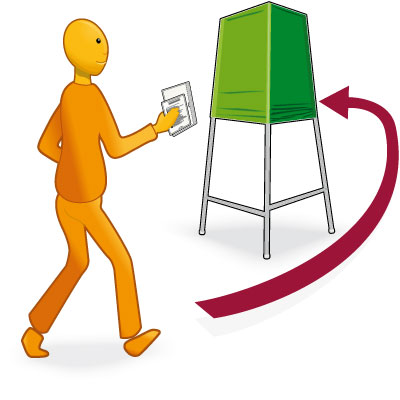
\includegraphics[width=\textwidth]{images/rosta.jpg}
	\end{column}
\end{columns}

\end{frame}

\begin{frame}{Tack för oss! Frågor?}

\begin{columns}
    \begin{column}{0.4\textwidth}
        \begin{itemize}
			\item Tack för att ni lyssnade!
			\item Har ni frågor?
		\end{itemize}
    \end{column}
	\begin{column}{0.6\textwidth}
    	\includegraphics[height=0.7\textheight]{images/interrobang.png}
	\end{column}
\end{columns}

\end{frame}

\clearpage
\begin{thebibliography}{9}

\bibitem{hac}
  Alfred J. Menezes, Paul C. van Oorschot and Scott A. Vanstone\\
  Handbook of Applied Cryptography.
  ISBN: 0-8493-8523-7\\
  CRC Press, Florida,
  5th Edition,
  2001.

\bibitem{oracle} 
   Mihir Bellare and Phillip Rogaway\\
   Random Oracles are Practical: A Paradigm for Designing Efficient Protocols\\
   ACM Conference on Computer and Communications Security 1993.

\bibitem{wikstrom1}
   Douglas Wikström\\
   How to Implement a Stand-alone Verifier for the Verificatum Mix-Net\\

\bibitem{wikstrom2}
  Lecture 08 DD2448
  http://www.csc.kth.se/utbildning/kth/kurser/DD2448/krypto13/handouts/lec08.pdf

\bibitem{mixnets}
   Philippe Golle, Markus Jakobsson, Ari Juels and Paul Syverson\\
   Universal Re-encryption for Mixnets\\
   Topics in Cryptology – CT-RSA 2004

   http://www.rsa.com/rsalabs/staff/bios/ajuels/publications/universal/Universal.pdf


\bibitem{mixnets2}
http://www.ee.washington.edu/research/nsl/papers/proceedings-06.pdf

\bibitem{electronicvoting}
  http://courses.csail.mit.edu/6.897/spring04/L17.pdf

\bibitem{electronicvoting2}
  http://courses.csail.mit.edu/6.897/spring04/L18.pdf

\bibitem{terelius}
http://www.nada.kth.se/~dog/research/TW10Conf.pdf

\bibitem{shoup}
http://cs.nyu.edu/courses/spring07/G22.3220-001/lec3.pdf


\end{thebibliography}


\end{document}
